\documentclass[11pt]{article}
\usepackage[utf8]{inputenc}
\usepackage{graphicx}
\usepackage{subfig}
\usepackage{enumerate}
\usepackage{amsmath}
\usepackage[letter, width=150mm, top=30mm, bottom=30mm]{geometry}
\usepackage[font={footnotesize}]{caption}
\usepackage[labelfont=bf]{caption}
\usepackage[english]{babel}

\setlength{\parskip}{1em}
\graphicspath{{../figs/}}

\title{Practice Session 01: Griffith Crack Theory: Aircraft Failure}
\author{Prithvi Thakur}
\date{Jan 23, 2019}

\begin{document}

\maketitle

% Problem 1
\section*{Griffith's energy balance}
The total surface energy due to a crack of length $a$ and a surface energy per unit length $\gamma$ is:
\begin{align}
    S &= 2\gamma a
\end{align}

The total strain energy for a circular crack is:
\begin{align}
    U = -\frac{\sigma}{2E}.\pi a^2
\end{align}

To estimate the crack length beyond which crack grows by lowering the system's energy, we set the derivative of the total energy with respect to crack length to zero:
\begin{align}
    \frac{\partial (S+U)}{\partial a} &= 2\gamma - \frac{\sigma_f^2}{E}\pi a^2 = 0 \\
    \sigma_f &= \sqrt{\frac{2E\gamma}{\pi a}} \\
    \implies a &= \frac{2E\gamma}{\pi \sigma_f^2} \\
    \implies a &= \frac{G_{Ic}E}{\pi \sigma_f^2}
\end{align}

Here, $a$ would give the critical crack length for spontaneous failure for a given strain energy release rate $G_{Ic}$ and given elastic modulus $E$.

\section*{Minimum crack length and choice of material}
The aircraft body is made out of Aluminium alloy because it is very light weight and can withstand high load. The windows will be made of glass but due to the rubber around the windows, we can assume that the stresses will not be transferred between the body of the aircraft and the glass windows. Therefore, we need to estimate the minimum crack length for Aluminium using the Griffith's energy balance approach, Eq. (5).
Given properties for Aluminium:
\begin{align}
    E &= 69\ GPa \\
    G_{Ic} &= 20\ kJm^{-2} \\
    \sigma_f &= 140\ MPa
\end{align}

Thus, the minimum crack length $a_c$ would be:
\begin{align}
    a_c &= \frac{20.10^{3} \times 69.10^9}{\pi \times 140^2.10^{12}} \\
    \implies a_c &= 2.2\ cm
\end{align}

Thus, if we observe a crack length of $2.2\ cm$ or greater in the aircraft body, we should not get in that aircraft.

Some materials in the aircraft like the engine and fan may be made out of steel, and using the same formula as above, we estimate the critical crack length for steel to be $36\ cm$.

\begin{figure}[!htb]
    \centering
    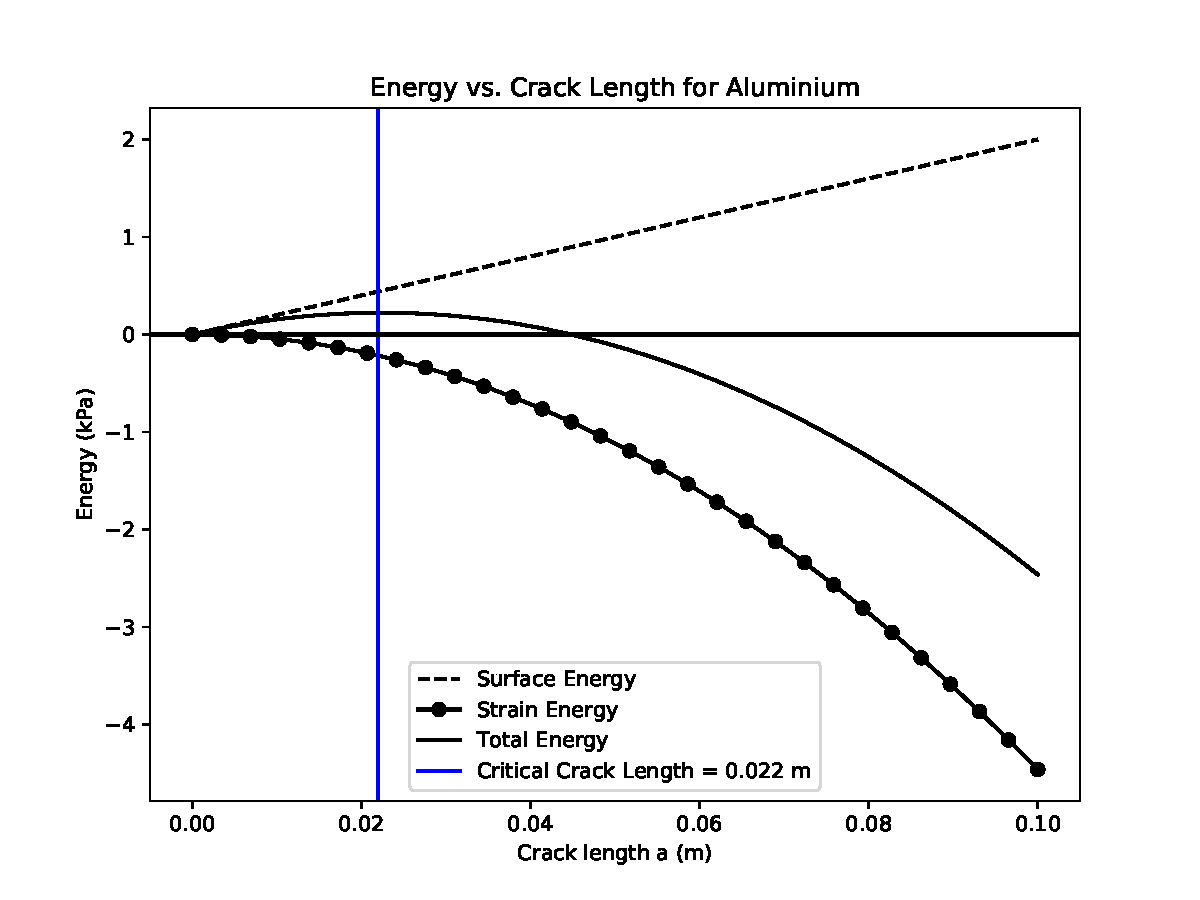
\includegraphics[scale=0.6]{fig1.pdf}
    \caption{Griffith's energy balance: Surface energy, strain energy, and total energy as a function of crack length for Aluminium. We see that the critical crack length is when the total energy of the system starts decreasing.}
\end{figure}

% Problem 2

\end{document}
